\headline{{\textbf{\Large\sffamily Trimmed Perspectives:}}\\
          {\textbf{\large\sffamily The Bonsai Critique Corner}}}
\label{2024-12-critique}
%\showthe\columnwidth
\begin{window}[%
    0,r,%
    \begin{minipage}{2.21in}%
        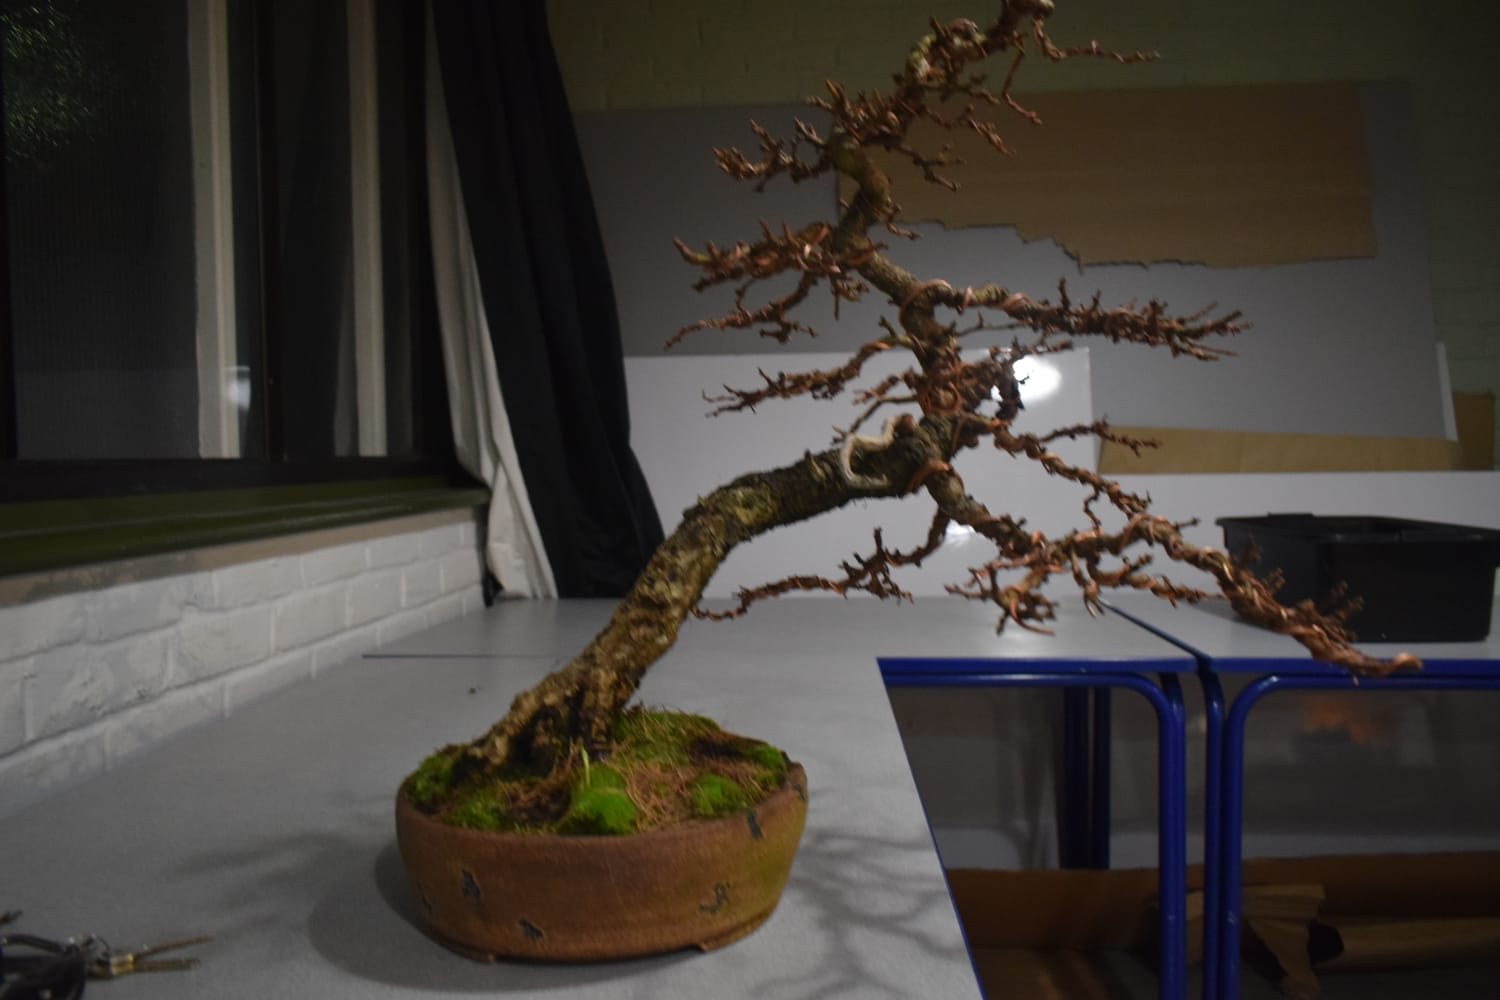
\includegraphics[width=2.21in]{2024_12/res/critique}%
    \end{minipage},%
    \centerline{\emph{A specimen under critique.}}%
]
    \noindent
    The recent \textbf{Tree Critique Corner} at the Twickenham Bonsai Club was a refreshing and insightful experience, thanks to the format change introduced after the AGM.
    Gone were the bustling plenary discussions; instead, we were treated to a more serene and focused setting, allowing members to engage deeply with the trees under scrutiny.
    %The shift was met with enthusiasm, and the quieter format seemed to bring out the best in both participants and the trees.
\end{window}

The session was ably coordinated by \textbf{Dave C.}, whose thoughtful approach and keen eye guided us through an in\--depth analysis of very different specimens.
Each critique felt constructive and uplifting, a testament to the supportive nature of the club.
By the end of the session, it was clear the new format was a resounding success.
Attendees left with fresh ideas and a deeper appreciation for the artistry involved in bonsai, proving that sometimes, a quieter approach yields the loudest inspiration.
We will cover next corner in more details!

%  Both trees demonstrated the beauty of bonsai at different stages of development---one refined, one emerging, yet both equally captivating.
%  What stood out most during the evening was the sense of camaraderie and inspiration that filled the room.

% First up was \textbf{Brian's Field Maple}, a tree that has reached an impressive stage of refinement.
% Its beautifully tapered trunk and well-balanced canopy spoke of years of dedicated care.
% Adam highlighted its subtle strengths, such as the harmonious branching and naturalistic flow, while also suggesting minor adjustments to enhance its already elegant composition.

% Next was \textbf{Cody's European Larch}, a tree in the early stages of its bonsai journey.
% Recently styled for the first time, the larch showed great promise with its dynamic movement and bold structure.
% Adam commended Cody for his vision and skill in capturing the tree’s potential.
% Though still raw compared to the Field Maple, the larch served as a brilliant reminder that every great bonsai begins with a daring first step.

\closearticle
